\documentclass[a4paper,12pt]{article}
\usepackage[utf8]{inputenc}
\usepackage[T1]{fontenc}
\usepackage[serbian]{babel}
\usepackage{amsmath}
\usepackage{graphicx}
\usepackage{geometry}
\geometry{margin=1in}
\title{Klasifikacija zvezda od galaksija korišćenjem klasifikacionih algoritama}
\author{\\Aleksa Toroman 84/2018 & Milica Sudar 79/2017 \\\\ Univerzitet u Beogradu, Matematički fakultet}

\begin{document}

\maketitle

\newpage
\renewcommand{\contentsname}{Sadržaj}
\tableofcontents

\newpage

\section{Uvod}
Klasifikacija nebeskih objekata na zvezde i galaksije predstavlja jedan od ključnih izazova u astronomiji i astrofizici. Tačna klasifikacija ovih objekata omogućava bolje razumevanje strukture i evolucije svemira. U ovom radu istražujemo primenu različitih klasifikacionih algoritama za predikciju da li je nebeski objekat zvezda ili galaksija na osnovu dostupnih podataka.\\
Cilj ovog istraživanja je da se primenom različitih klasifikacionih algoritama postigne visoka tačnost u klasifikaciji, kao i da se identifikuju ključni atributi koji najviše doprinose tačnosti predikcija. Kroz rad ćemo se osvrnuti na metodologiju korišćenu u analizi, opis podataka, implementaciju algoritama, analizu rezultata i zaključke do kojih smo došli.

\section{Metodologija}
\subsection{Softverski alati i okruženje}
Za potrebe ovog istraživanja korišćeni su sledeći softverski alati i okruženja:
\begin{itemize}
    \item \textbf{PyCharm}: Integrisano razvojno okruženje (IDE) za Python, koje omogućava efikasno kodiranje, debugovanje i testiranje.
    \item \textbf{Python}: Glavni programski jezik korišćen za implementaciju algoritama, analizu podataka i vizualizaciju rezultata.
    \item \textbf{Jupyter Notebook}: Interaktivno okruženje za analizu podataka i vizualizaciju, koje omogućava lako eksperimentisanje sa kodom i pregled rezultata.
\end{itemize}

\subsection{Korišćene biblioteke}
Za analizu podataka i implementaciju klasifikacionih algoritama korišćene su sledeće Python biblioteke:
\begin{itemize}
    \item \textbf{pandas}: Za manipulaciju i analizu podataka.
    \item \textbf{numpy}: Za numeričke operacije i rad sa nizovima.
    \item \textbf{scikit-learn}: Za implementaciju i evaluaciju klasifikacionih algoritama.
    \item \textbf{matplotlib} i \textbf{seaborn}: Za vizualizaciju podataka i rezultata.
\end{itemize}


\section{Podaci i Pretprocesiranje}
U ovom istraživanju razmatrana su dva različita skupa podataka: jedan sa SuperCOSMOS Sky Survey sajta i drugi sa Sloan Digital Sky Survey sajta. U nastavku ćemo opisati način prikupljanja, učitavanja i pretprocesiranja podataka za oba skupa.

\subsection{SuperCOSMOS Sky Survey}
Podaci sa SuperCOSMOS Sky Survey sajta prikupljeni su korišćenjem dostupnih pretraga i alata za ekstrakciju podataka dostupnih na zvanicnom sajtu. Originalno, skup podataka je sadržao 901,322 redova i 43 atributa, međutim deo atributa koji je bio bitan za proces klasifikacije je imao određene nedostatke.

Tokom pretprocesiranja podataka identifikovano je nekoliko značajnih problema:
\begin{itemize}
    \item \textbf{Magnituda}: Mnoge vrednosti za magnitude (u, g, r, i, z) su bile prazne ili su imale placeholder vrednosti koje su bile velike cifre, što je indiciralo nedostatak stvarnih podataka ili prisustvo grešaka. Ove vrednosti su morale biti odstranjene pre dalje analize.
    \item \textbf{RA i DEC}: Vrednosti za Celestial Right Ascension (RA) i Celestial Declination (DEC) su bile vrlo slične za sve redove, što je ukazivalo na to da su podaci dobijeni sa ograničenog područja neba. Ovo je bilo posledica limitacije upita  koji je vraćao podatke samo iz određenih regiona sa definisanim radijusom pretrage.
\end{itemize}

Nakon uklanjanja nedostajućih vrednosti i outlier-a, preostalo je svega 80,000 redova za dalju analizu, što je znatno manje od originalnih 1,000,000 redova. Ovo smanjenje broja redova je posledica visokog procenta nedostajućih vrednosti i prisustva placeholder-a koji su značajno umanjili kvalitet podataka.

\subsection{Sloan Digital Sky Survey}
Podaci sa Sloan Digital Sky Survey (SDSS) sajta prikupljeni su korišćenjem odgovarajućeg SQL upita na njihovom data centru. Upit je konstruisan kako bi se dohvatili svi relevantni atributi za vizualizaciju i treniranje klasifikacionog modela.

\begin{figure}[h!]
\centering
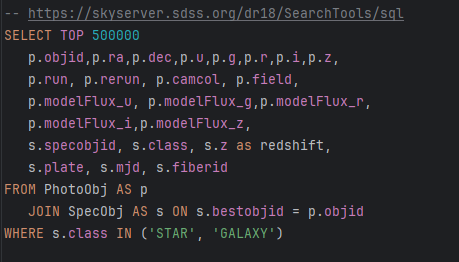
\includegraphics[width=0.8\textwidth]{sql.png}
\caption{SQL upit korišćen za prikupljanje podataka sa SDSS sajta}
\label{fig:sql_query}
\end{figure}

Ovim upitom dohvaćeno je 500,000 redova, obuhvatajući sve potencijalno bitne atribute za dalju analizu. Spektar atributa koji je dostupan putem SDSS baze podataka je značajno veći u odnosu na SuperCOSMOS, što omogućava bogatiju analizu i bolje treniranje modela. Istraživanjem šeme podataka u SDSS bazi, identifikovan je veći broj atributa koji mogu biti korisni za klasifikaciju.\\\\
S obzirom na to da je klasifikacija u ovom istraživanju fokusirana na razlikovanje zvezda i galaksija, eksplicitno smo tražili da se dohvate podaci koji uključuju samo one klase objekata koje pripadaju ili zvezdama ili galaksijama, isključujući quasare kao tip nebeskih objekata.\\\\
Pretprocesiranje podataka sa SDSS sajta pokazalo je znatno manji broj nedostajućih vrednosti i outlier-a u poređenju sa SuperCOSMOS Sky Survey skupom podataka. Nakon čišćenja podataka, preostalo je oko 492,000 redova koji su bili kvalitetni za dalju analizu. S obzirom na viši kvalitet podataka kao i veći broj slogova, dalji rad i analiza u ovom istraživanju fokusirani su na ovaj skup podataka.

\subsection{Odabrani Atributi za Treniranje Modela}

Za treniranje klasifikacionih modela korišćeni su sledeći atributi: 'ra', 'dec', 'u', 'g', 'r', 'i', 'z', 'class', 'redshift'. Ovi atributi su pažljivo odabrani na osnovu njihove relevantnosti u astrofizici i njihove sposobnosti da pomognu u razlikovanju zvezda i galaksija.

\begin{itemize}
    \item \textbf{RA (Right Ascension)}: Ovo je jedna od dve osnovne nebeske koordinate koje se koriste za određivanje položaja nebeskih objekata na nebeskoj sferi. RA se meri u satima, minutima i sekundama, i predstavlja ugaonu udaljenost objekta istočno od Prolećne tačke. RA je ekvivalent geografskoj dužini na Zemlji.
    
    \item \textbf{DEC (Declination)}: Druga osnovna nebeska koordinata koja se koristi za određivanje položaja objekata na nebeskoj sferi. DEC se meri u stepenima, minutima i sekundama, i predstavlja ugaonu udaljenost objekta severno ili južno od nebeskog ekvatora. DEC je ekvivalent geografskoj širini na Zemlji.
    
    \item \textbf{Magnituda (u, g, r, i, z)}: Magnituda je mera sjaja nebeskog objekta viđenog sa Zemlje. Postoji pet filtera (u, g, r, i, z) koji mere sjaj u različitim delovima elektromagnetnog spektra:
    \begin{itemize}
        \item \textbf{u (ultraljubičasti filter)}: Mera sjaja u ultraljubičastom delu spektra.
        \item \textbf{g (zeleni filter)}: Mera sjaja u zelenom delu spektra.
        \item \textbf{r (crveni filter)}: Mera sjaja u crvenom delu spektra.
        \item \textbf{i (bliski infracrveni filter)}: Mera sjaja u bliskom infracrvenom delu spektra.
        \item \textbf{z (daleki infracrveni filter)}: Mera sjaja u dalekom infracrvenom delu spektra.
    \end{itemize}
    
    \item \textbf{Class (klasa)}: Ovaj atribut označava klasifikaciju objekta kao zvezda ili galaksija. Ovo je ciljna promenljiva u klasifikacionom modelu.
    
    \item \textbf{Redshift}: Crveni pomak je ključan fenomen u astronomiji jer omogućava određivanje udaljenosti i brzine udaljavanja nebeskih objekata, što je posebno važno za klasifikaciju između zvezda i galaksija. Razumevanje crvenog pomaka pomaže u identifikaciji galaksija koje se udaljavaju od nas zbog širenja svemira, dok zvezde, sa svojim karakterističnim relativnim brzinama unutar naše galaksije, pružaju dodatne informacije o njihovim kretanjima i položajima u odnosu na Sunčev sistem.
\end{itemize}

Atributi kao što su 'objid', 'run' i 'rerun' odnose se na administraciju podataka i nisu direktno bitni za izradu samog klasifikacionog modela. Atributi 'camcol', 'field', 'plate' i 'fiberid' predstavljaju tehničke podatke koji se odnose na uslove pod kojima je snimljen nebeski objekat. Atribut 'mjd' predstavlja modifikovani Julianov datum posmatranja i nije relevantan za određivanje da li je objekat zvezda ili galaksija.

Odabir ovih atributa omogućava modelima da imaju dovoljno informacija za preciznu klasifikaciju nebeskih objekata. RA i DEC pružaju informacije o položaju objekta na nebu, magnitude u različitim filterima omogućavaju analizu sjaja objekta u različitim delovima spektra, klasa objekta je cilj klasifikacije, dok crveni pomak pruža dodatne informacije o udaljenosti i brzini objekta.

\subsection{Učitavanje i Čišćenje Podataka}


\subsubsection{Učitavanje Podataka}
Podaci su učitani korišćenjem biblioteke pandas, koja je moćan alat za manipulaciju i analizu podataka u Pythonu. Nakon učitavanja, proverili smo da li je skup podataka uspešno dovučen i uradili smo osnovne operacije za pregled podataka i njegove statistike. Takođe u ovom procesu su i isključene kolone koje nisu potrebne za dalju analizu i treniranje modela za klasifikaciju:


\begin{figure}[h!]
\centering
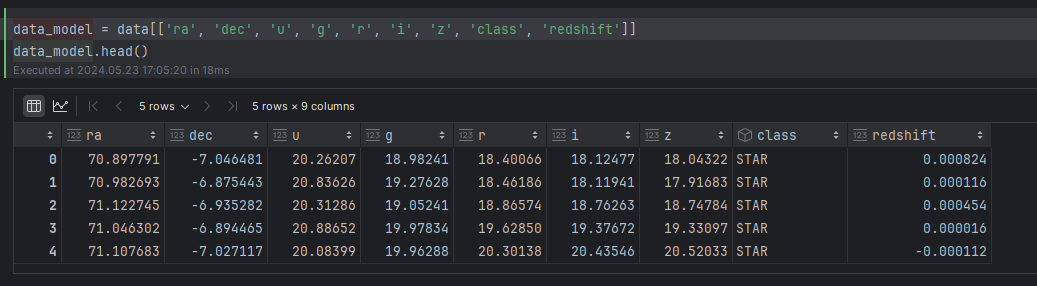
\includegraphics[width=0.8\textwidth]{list_data.png}
\caption{Izlistavanje nekolicine redova učitanog skupa podataka}
\label{fig:sql_query}
\end{figure}

\clearpage

\subsubsection{Identifikacija i Uklanjanje Anomalija}
Proces čišćenja podataka je ključan korak u pripremi podataka za treniranje modela. Ovaj proces uključuje identifikaciju i uklanjanje anomalija i outlier-a i razrešavanje praznih vrednosti.\\\\
Prvo smo proverili da li skup podatak ima nedostajuće vrednosti u nekim kolonama:

\begin{figure}[h!]
\centering
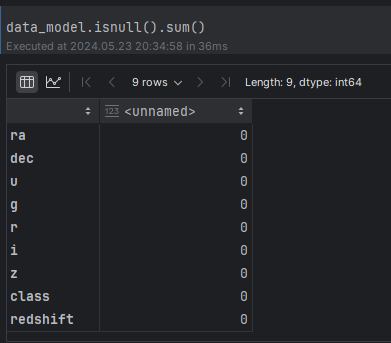
\includegraphics[width=0.8\textwidth]{null_column_check.png}
\caption{Provera nedostajućih vrednosti u kolonama}
\label{fig:sql_query}
\end{figure}

Međutim, naš skup podataka nije imao takav slučaj pa smo obradu ovakvih redova preskočili.\\\\
Za uklanjanje outlier-a koristili smo algoritam Local Outlier Factor (LOF) za identifikaciju i uklanjanje outlier-a. LOF algoritam procenjuje udaljenost svakog podatka od njegovih suseda i identifikuje one podatke koji se značajno razlikuju od ostatka skupa.\\\\
Takođe, i bez algoritma jednostavnim pregledom osnovih statistika smo uvideli da neke kolone u sebi imaju određene anomalije:\\\\

\clearpage

\begin{figure}[h!]
\centering
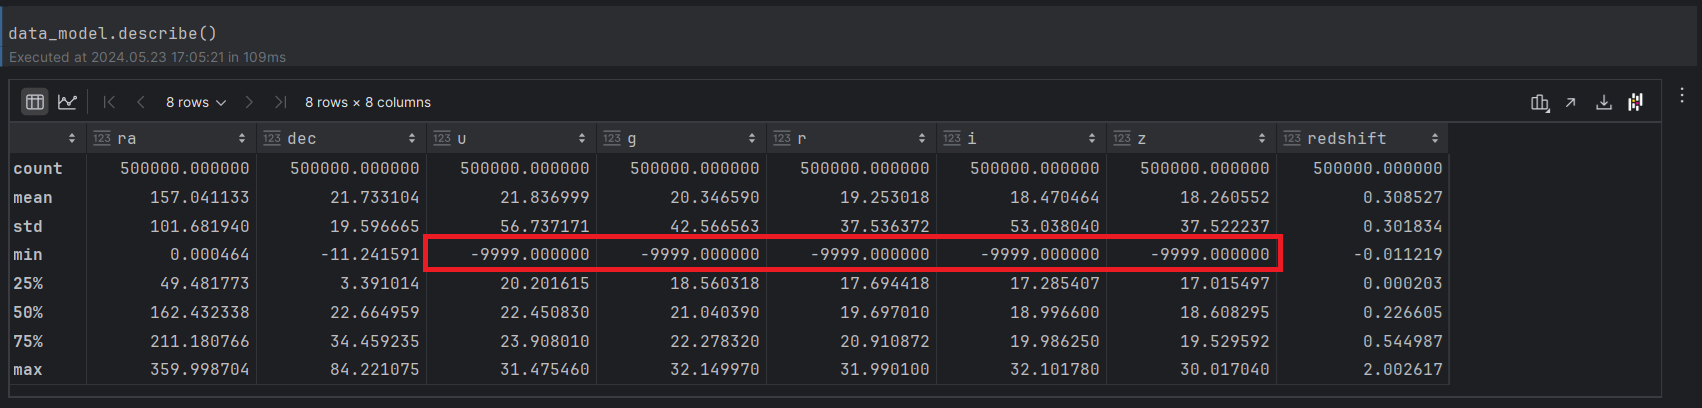
\includegraphics[width=0.8\textwidth]{data_model_anomalies.png}
\caption{Prikaz osnovne statistike skupa podataka}
\label{fig:sql_query}
\end{figure}

Na slici se vidi da određeni broj kolona koji se odnosi na magniture ima vrednost od -9999.00 što je predstavljalo placeholder za redove koje imaju grešku ili su nepoznate.\\\\
Koraci u procesu čišćenja podataka uključivali su:
\begin{itemize}
    \item \textbf{Provera atributa}: Prvo je provereno da li skup podataka sadrži kategoričke atribute. Pošto su svi atributi numerički, svi atributi su uključeni u primeni algoritma za detekciju outlier-a.
    \item \textbf{Filtriranje outlier-a}: Na osnovu rezultata LOF algoritma, podaci identifikovani kao outlier-i su uklonjeni iz skupa podataka.
\end{itemize}
Korišćenjem ovog pristupa, uspeli smo da identifikujemo i uklonimo outlier-e iz skupa podataka, čime smo poboljšali kvalitet podataka za treniranje modela. Nakon čišćenja podataka, preostalo je 492,153 redova koji su bili kvalitetni za dalju analizu.

\begin{figure}[h!]
\centering
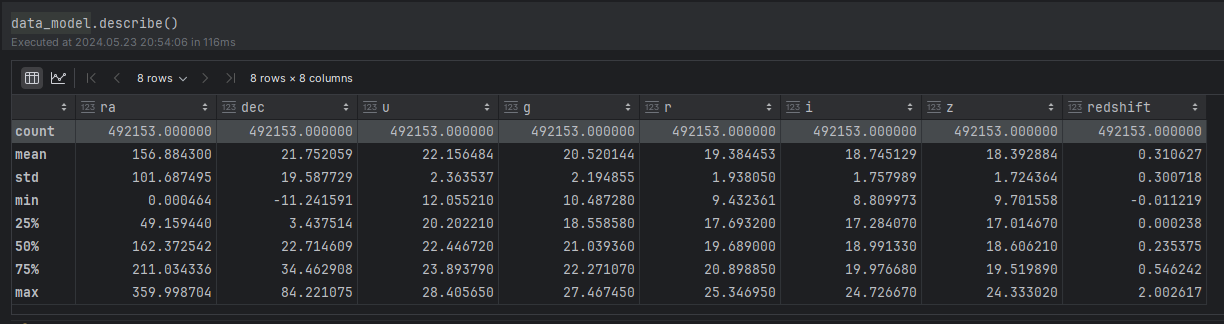
\includegraphics[width=0.8\textwidth]{data_model_filtered.png}
\caption{Skup podataka nakon uklanjanja outlier-a}
\label{fig:sql_query}
\end{figure}

\subsection{Vizualizacija i razumevanje podataka}

\section{Algoritmi}

\subsection{Slučajne šume}
Opis teorije i implementacije.

\subsection{Stabla odlučivanja}
Opis teorije i implementacije.

\section{Analiza rezultata}


\subsection{Trening i test skupovi}

\subsection{Performanse modela}

\section{Zaključak}


\begin{thebibliography}{9}
\bibitem{data_mining}
\end{thebibliography}

\end{document}
